%%%%%%%%%%%%%%%%%%%%%%%%%%%%%%%%%%%%%%%%%%%%%%%%%%%%%%%%%%%%%%%%%%% 
%% Desarrollo -  Modelado en punto fijo
%%%%%%%%%%%%%%%%%%%%%%%%%%%%%%%%%%%%%%%%%%%%%%%%%%%%%%%%%%%%%%%%%%%

\subsection{Modelo en punto fijo}
\begin{frame}
  \frametitle{\textbf{Tabla de Contenidos}}
  \begin{center}
    {\vspace{-1.5cm}\Large \textbf{Sección \thesection: \secname }\vspace{0.5cm}}
    \begin{beamercolorbox}[
      sep=8pt,center]{part title}
      \usebeamerfont{part title}
      \textbf{\subsecname}
    \end{beamercolorbox}
  \end{center}
\end{frame}

\begin{frame}
  \frametitle{\textbf{Consideraciones}}
   \framesubtitle{\secname : \subsecname}

    \begin{block}{\centering \textbf{Calculo de intervalos}}
    \begin{itemize}\small
    \item El calculo del intervalo de entrada se realiza a la mitad de frecuencia que el de salida en el bloque codificador, de forma inversa en el decodificador.
     \item El cálculo del intervalo de entrada y salida del codificador se realiza de manera recursiva y secuencial respectivamente.
    \item El cálculo del intervalo de entrada y salida del decodificador se realiza de forma recursiva.
    \end{itemize}
    \end{block}
    \vspace{-0.2cm}

    \begin{block}{\centering \textbf{Cuantizacion de variables}}
    Se consideran tres grupos de variables:
    \begin{itemize}\small
    \item Intervalos del codificador.
    \item Probabilidades.
    \item Intervalos del decodificador.
    \end{itemize}
    \end{block}
\end{frame}

\begin{frame}
  \frametitle{\textbf{Resoluciones de intervalos del codificador}}
      \framesubtitle{\secname : \subsecname}

    \begin{block}{}
    \begin{itemize}
    \item Se cuantizan únicamente los limites de los intervalos del codificador.
    \item La resolución elegida para este grupo de variables será U(7,6).
    \end{itemize}
    \end{block}
    \vspace{-0.3cm}
    \begin{columns}
    \begin{column}{0.48\paperwidth}
     \begin{figure}
     \centering
    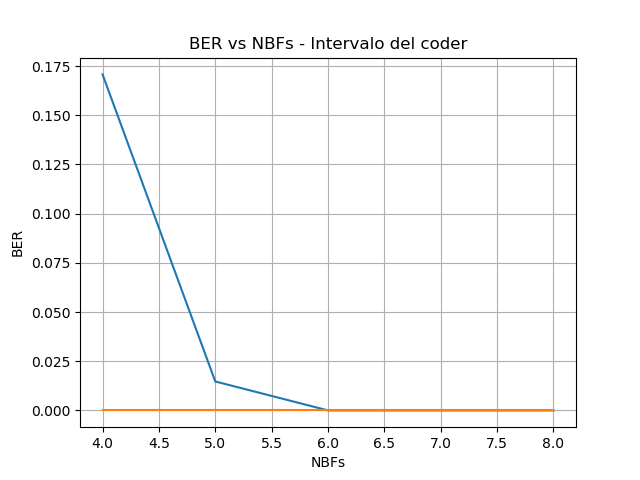
\includegraphics[width=\textwidth]{Graficos/cuantization.png}%
    \caption{Con escalado}
    \end{figure}
    \end{column}
    \begin{column}{0.48\paperwidth}  
    \begin{figure}
    \centering
    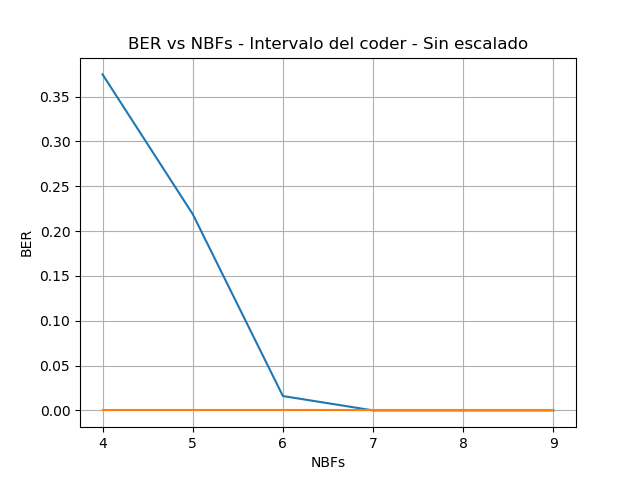
\includegraphics[width=\textwidth]{Graficos/cuantization4.png}%
    \caption{Sin escalado}
    \end{figure}
    \end{column}
\end{columns}
    \end{frame}

\begin{frame}
  \frametitle{\textbf{Resolución de probabilidades}}
\framesubtitle{\secname : \subsecname}
    \begin{block}{}
    \begin{itemize}
    \item  La resolución de los intervalos del codificador se mantiene constante.
    \item  La resolución elegida para este grupo de variables será U(5,4).
    \end{itemize}
    \end{block}
       \vspace{-0.3cm}
    \begin{columns}
    \begin{column}{0.48\paperwidth}
     \begin{figure}
     \centering
    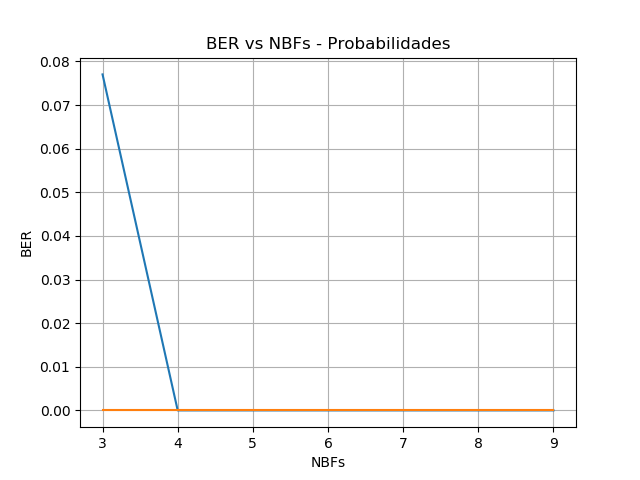
\includegraphics[width=\textwidth]{Graficos/cuantization2.png}%
    \caption{Con escalado}
    \end{figure}
    \end{column}
    \begin{column}{0.48\paperwidth}  
    \begin{figure}
    \centering
    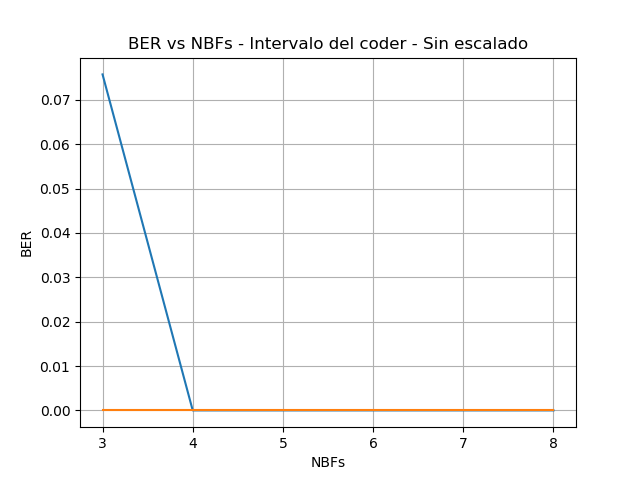
\includegraphics[width=\textwidth]{Graficos/cuantization5.png}%
    \caption{Sin escalado}
    \end{figure}
    \end{column}
\end{columns}
   \end{frame}

\begin{frame}
  \frametitle{\textbf{Resolución de intervalos del decodificador}}
\framesubtitle{\secname : \subsecname}

    \begin{block}{}
    \begin{itemize}
    \item Se mantiene constante la resolución de los intervalos del codificador y las variables de probabilidad.
    \item La resolución elegida para este grupo es U(10,9).
    \end{itemize}
    \end{block}
    \vspace{-0.3cm}
    \begin{columns}
    \begin{column}{0.48\paperwidth}
     \begin{figure}
     \centering
    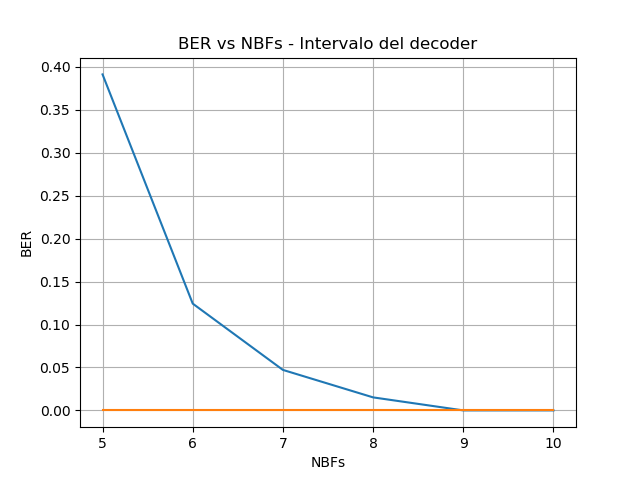
\includegraphics[width=\textwidth]{Graficos/cuantization3.png}%
    \caption{Con escalado}
    \end{figure}
    \end{column}
    \begin{column}{0.48\paperwidth}  
    \begin{figure}
    \centering
    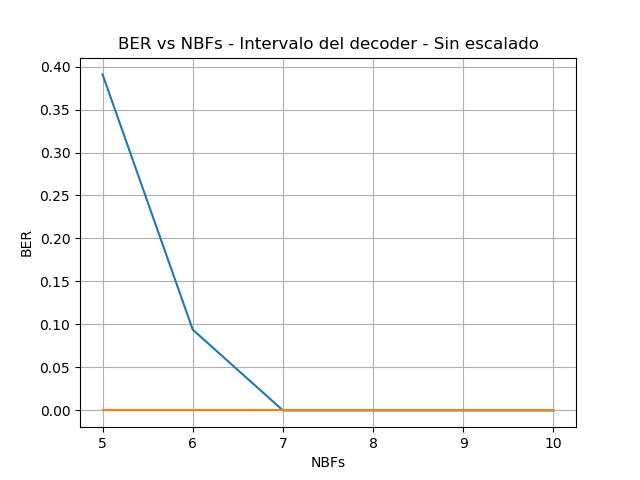
\includegraphics[width=\textwidth]{Graficos/cuantization6.png}%
    \caption{Sin escalado}
    \end{figure}
    \end{column}
\end{columns}
\end{frame}

\begin{frame}
  \frametitle{\textbf{Consideraciones finales}}
    \framesubtitle{\secname : \subsecname}

    \begin{block}{\centering \textbf{Retardos en la salida del codificador}}
     \begin{itemize}
     \item Se deben incluir de tal forma que no afecte el sincronismo de datos.
      \item Se agregó una cantidad de retardos en el canal de comunicación para que esto no sea un problema.
      \end{itemize}
     \end{block}
    \begin{block}{\centering \textbf{Ejemplo}}
    La secuencia [1,0,0,0] se codifica a [0,1,0,0,0,0,1,0], si el canal presenta un retardo, la secuencia será [1,0,0,0,1,0,0,0] y decodificacion resultara erronea. 
    \end{block}
\end{frame}



